\begin{figure}[t]
\centering
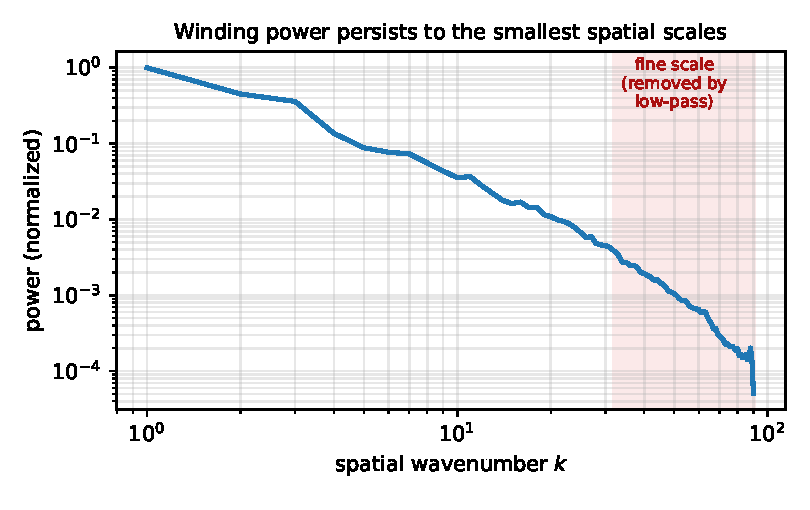
\includegraphics[width=0.6\textwidth]{figures/fig_psd.pdf}
\caption[Spatial power spectrum]{\textbf{Winding power persists to the smallest
spatial scales.} Radially-averaged spatial power spectrum of the asinh winding
field, averaged over active regions and normalised to the largest scale. Power
falls off only gradually with wavenumber and never reaches a flat noise floor:
there is real structure at every scale. Combined with the temporal incoherence of
those small scales (Figure~\ref{fig:autocorr}), this justifies removing the
fine-scale band (shaded) by low-pass before forecasting.}
\label{fig:psd}
\end{figure}
